\documentclass[twoside,11pt]{article}

% Any additional packages needed should be included after jmlr2e.
% Note that jmlr2e.sty includes epsfig, amssymb, natbib and graphicx,
% and defines many common macros, such as 'proof' and 'example'.
%
% It also sets the bibliographystyle to plainnat; for more information on
% natbib citation styles, see the natbib documentation, a copy of which
% is archived at http://www.jmlr.org/format/natbib.pdf

\usepackage{jmlr2e}
\usepackage{cite}
\usepackage{listings}
\usepackage{caption}
\usepackage{subcaption}
\usepackage{float}

%definitios for source code
\lstset{ %
basicstyle=\footnotesize
}

% Definitions of handy macros can go here

\newcommand{\dataset}{{\cal D}}
\newcommand{\fracpartial}[2]{\frac{\partial #1}{\partial  #2}}

% Heading arguments are {volume}{year}{pages}{submitted}{published}{author-full-names}

\jmlrheading{todo}{2017}{todo}{todo}{todo}{marvin}{Lucas B. Miguel et al}

% Short headings should be running head and authors last names

\ShortHeadings{Marvin - From exploratory models to production}{}
\firstpageno{1}

\begin{document}

\title{Marvin - From exploratory models to production}

\author{\name Lucas B.\ Miguel \email lucas.bonatto@b2wdigital.com
       \AND
        \name Daniel Takabayashi \email daniel.takabayashi@b2wdigital.com
       \AND
       \name Jose R.\ Pizani \email jose.pizani@b2wdigital.com
       %\addr Tech Labs - B2W Digital
       \AND
       \name Tiago Andrade \email tiago.andrade@b2wdigital.com
       \AND
       \name Brody West \email brodyw@mit.edu \\
       }

\editor{Claire Hardgrove, Keiran Thompson and Louis Dorard}

\maketitle

\begin{abstract}%   <- trailing '%' for backward compatibility of .sty file
Marvin is an open source project that focuses on empowering data science teams to deliver complex solutions supported by a high-scale, low-latency, language agnostic and standardized architecture platform, while simplifying the process of exploration and modeling. Build model-dependent applications in a robust way is not trivial, one is required to have knowledge in advanced areas of sciences like computing, statistics and math. Marvin aims to abstract the complexities in the creation process of a scalable, high available, interoperable and maintainable software.
\end{abstract}

\begin{keywords}
  Machine Learning, Platform, Predictive Analytics, Artifical Intelligence
\end{keywords}

\section{Introduction}

Being able to quickly identify hidden patterns in datasets and wisely choose the best model to train historical data and make predictions are the biggest advantage of data-driven organizations against their competitors. Knowing the customer demand for a product before buying it~\citep{chen2000quantifying} or being able to detect a fraud before charging the customer's credit card~\citep{chan1998toward} with a certain level of confidence are examples of how companies doing businesses on the internet are making better decisions and maximizing their earnings.

Capturing and storing large amounts of data is a commonplace for most companies these days. Having more data available is often a positive aspect in order to train models with a lower error rate. However, writing code to effectively process terabytes of data and provide near-real-time predictions supporting high throughput is not a trivial task. One is required to have knowledge in advanced areas of science, such as computing, statistics and math. High scale data processing frameworks~\citep{zaharia2010spark} fulfill their role by abstracting some of the complexities related to distributed computing and process orchestration. Libraries like MLLib~\citep{meng2015ml} and scikit-learn~\citep{pedregosa2011scikit} facilitate it by providing high level interfaces to common machine learning algorithms. Even so, building robust model-dependent applications is tricky and requires specialized knowledge. There is an open space for a platform that empowers the data scientist with the tools and abstractions needed to create scalable, high available, interoperable and maintainable predictive software. 

In this paper we present Marvin, an open source platform that aims to help data scientists on several tasks during the life cycle of an artificial intelligence project. In section 2 we describe the platform main features, section 3 contains implementation details, section 4 has a sample application and finally in section 5 we summarize our findings.

\section{Marvin Overview}

A model-dependent application is described by an application that processes historical data and train a mathematical model such that the output $Y$ can be explained by the different values of the input $X$. Some categories of algorithm in the artificial intelligence area fits in this description, e.g. machine learning, natural language processing, computer vision. Marvin provide tools that will help in different phases of a project with such characteristics. The tools can be executed both on-premise or in a cloud infrastructure, giving the flexibility that is needed for different scenarios. Marvin is different from ML PaaS~\citep{pmlr-v50-azureml15}, since it can be executed on-premise and allow the use of any algorithm that can be implemented in general-purpose languages~\citep{van2003python}~\citep{odersky2004scala}. In fact, Marvin could be used as the back-end of such type of platforms.

Marvin was built to enforce the pillars of the basic phases of a model development project, see Figure \ref{fig_cycle}. 
\begin{figure}[h]
\centering
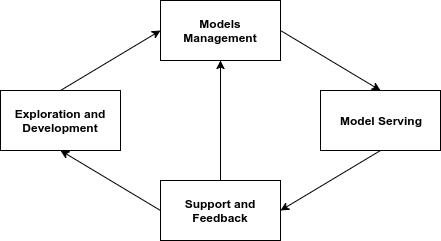
\includegraphics[scale=0.6]{fig/dev-cycle.png}
\DeclareGraphicsExtensions.
\caption{Model application development cycle.}
\label{fig_cycle}
\end{figure}

To achieve that, Marvin provide several features, those include:
\begin{enumerate}
    \item Toolbox - Provide a great set of common tools that are commonly used during the exploration phase of a data science projects and will eventually be carried up to production. The data scientist can take advantage of notebooks, plotting libraries, data frames and so on. 
    \item Experiment Versioning - During the exploration and exploitation of the problem it is common to test several hypothesis and eventually change approach. Keeping the history of experiments is useful and may serve to explain the final solution.
    \item Data Sync CLI - During the model development data is intensively accessed, either to perform feature engineering or backtest the model. In complex environments it's often not a good approach to access production databases during development phase. To solve that Marvin provide a tool to sample data from the official dataset and work locally.
    \item Unit Test Framework - In order to ensure a testable application, Marvin provides a built-in unit test framework, encouraging the data scientist to avoid bugs being introduced in the model application in the future.
    \item Project Generator - Marvin introduces a design pattern, see Figure \ref{fig_dase}, to ensure that applications will be built in a decoupled manner. The project generator utility creates the base skeleton for applications, the data scientist is required to only populate the skeleton files with their logic.
    \item Artifact Versioning - Marvin keeps track of artifacts generated during the training pipeline. When running the application in production Marvin allows the user to restore the system to a previous state, i.e. publishing a model trained last week because the current model is presenting greater error rate.
    \item Large Dataset Processing - Integration with main frameworks for parallel and distributed computing to allow the effective handling of large datasets.
    \item Training Pipeline Interface - The phases involved in the training pipeline (data acquisition, data preparation, training) can be started through the CLI or via REST HTTP calls. Allowing the application to be executed by external agents.
    \item Feedback Server - In order to allow the model to receive external stimulation, Marvin provides a feedback server. User and applications can send feedback data to the model, which can be interpreted and perharps start a new training.
    \item Predictor Server - When finishing the training pipeline Marvin persists the serialized model in a persistent memory storage. This model is loaded afterwards by the predictor server and is accessible via REST HTTP calls. Users and applications can then make predictions taking advantage of the model.
\end{enumerate}

Marvin is composed by three main components, see Figure \ref{fig_components}. The toolbox is both a command line interface and a library that contains a set of utilities to help data scientists during the phase of exploration and development. Using the toolbox the user will build his application, which in the context of Marvin is called an engine. The engine must be built following a design pattern proposed by Marvin, the toolbox will generate a scaffold with the classes corresponding to this pattern. Each phase in the pattern will produce an artifact, that can be persisted and reloaded. Lastly, the engine-executor is the component responsible by orchestrating the execution of engines and also by deploying servers to allow external interaction with it.

\begin{figure}[h]
\centering
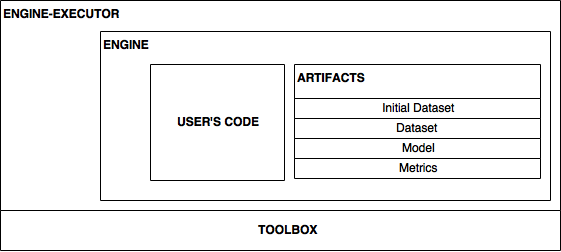
\includegraphics[scale=0.6]{fig/components.png}
\DeclareGraphicsExtensions.
\caption{Marvin components.}
\label{fig_components}
\end{figure}

Several previous work already help on the task of implementing artificial intelligence applications able to deal with large datasets and achieve good performance. SystemML~\citep{ghoting2011systemml} provide a high level declarative interface to implement machine learning applications that can process massive amounts of data. Pregel~\citep{malewicz2010pregel} introduces a computational model suitable for large-scale graph processing. OptiML~\citep{sujeeth2011optiml} is a domain-specific language (DSL) to achieve implicit parallelism on machine learning applications. MLI~\citep{sparks2013mli} offers an API for distributed machine learning that helps turning prototypes into industry-grade ML software. Although these works do a great job abstracting complexity in the batch processing phase, they do not intend to offer tools to help during problem exploration and model serving. Table \ref{table-comp} shows the comparison of Marvin, SystemML and a market solution~\citep{clouddsw}.


\begin{table}[!htbp]
\centering
\begin{tabular}{|l|c|c|l|}
\hline
                                  & \multicolumn{1}{l|}{\textbf{Marvin}} & \multicolumn{1}{l|}{\textbf{SystemML}} & \textbf{Cloudera DSW}  \\ \hline
Multi-language support            & x                                    & \multicolumn{1}{l|}{}                  & \multicolumn{1}{c|}{x} \\ \hline
HDFS support                      & x                                    & x                                      & \multicolumn{1}{c|}{x} \\ \hline
Distributed CPU ML API            & x                                    & x                                      &                        \\ \hline
Single node capability            & x                                    & x                                      &                        \\ \hline
Toolbox (development environment) & x                                    &                                        & \multicolumn{1}{c|}{x} \\ \hline
Templates                         & x                                    &                                        & \multicolumn{1}{c|}{x} \\ \hline
Integrated notebooks              & x                                    &                                        & \multicolumn{1}{c|}{x} \\ \hline
Models management                 & x                                    &                                        & \multicolumn{1}{c|}{x} \\ \hline
Data versioning control           & x                                    &                                        &                        \\ \hline
Pipeline scaffolding              & x                                    &                                        &                        \\ \hline
Unit test integration             & x                                    &                                        &                        \\ \hline
REST API                          & x                                    &                                        &                        \\ \hline
Pre-process optimization          &                                      & x                                      &                        \\ \hline
Feedback server          & x                                     &                                       &                        \\ \hline
\end{tabular}
\caption{Functionality comparison}
\label{table-comp}
\end{table}

\section{Implementation Details}

One of Marvin's main objective is to optimize execution of it's users' applications in order to process large datasets and allow a high number of concurrent model access without penalizing performance. To help users see the boundary of different executions flow within the application we propose the separation of actions in two categories:
\begin{itemize}
    \item batch - e.g. train, evaluate, prepare
    \item online - e.g. predict, feedback
\end{itemize}

Batch actions are executed asynchronously and the result of it's execution will be an artifact. They have this characteristic because they are expected to be data-intensive jobs. In order to achieve parallelism in different levels, Marvin applications run on top of common data processing frameworks, see Figure \ref{fig_spark}. The Marvin context is a component that frees the data scientist of setting up and optimizing the framework, it wraps some methods from the original framework library but also expose the main features of it.
\begin{figure}[h]
\centering
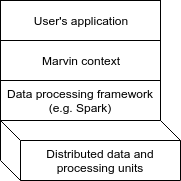
\includegraphics[scale=0.7]{fig/marvin-spark.png}
\DeclareGraphicsExtensions.
\caption{Multi-tier architecture for batch processing.}
\label{fig_spark}
\end{figure}

On the other hand, online actions are executed synchronously and they may generate a valid result. Their result will usually be interpreted by other application, therefore to ensure simple scalability, interoperability, availability and the needed consistency we adopted a microservice-based architecture~\citep{brewer2000towards}~\citep{fowler2014microservices}. 

All application's execution are orchestrated by the engine-executor component. This is a configurable component that can be deployed in different formats, depending on the environment complexity. One may want to deploy an engine-executor instance for each pipeline phase (data acquisition, data preparation, model training, etc.), it would avoid a single point of failure and allow independent scalability for each phase. However, projects on a smaller scale may prefer to deploy all the phases and the predictor server in the same instance. To achieve safe and effective concurrent execution, the underlying of engine-executor is implemented according to the Actor model~\citep{hewitt1973session}.

As we understand that there is no mother programming language for artificial intelligence applications, we built Marvin under the assumption that it should be language agnostic. It means that users are free to implement their applications using their preferred language, provided that its support is implemented. Figure \ref{fig_rpc} shows how Marvin is using the RPC~\citep{srinivasan1995rpc} protocol to execute code written in different languages.

\begin{figure}[h]
\centering
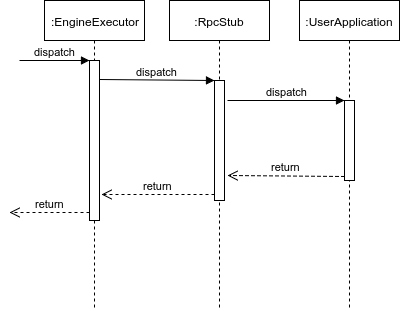
\includegraphics[scale=0.5]{fig/marvin-rpc.png}
\DeclareGraphicsExtensions.
\caption{Simplified sequence of engine-executor executing online action on user's code.}
\label{fig_rpc}
\end{figure}

\subsection{Performance Evaluation}

Aiming to evaluate the parallelism ability of the predictor server, we conducted a set of experiments predicting classes of iris in a Support Vector Machine (SVM)~\citep{hearst1998support} model trained using the classical Fisher's iris dataset~\citep{fisher1936use} for classification. The overall objective of this experiment was to ensure that the predictor server is able to take advantage of multi-core architectures while not impacting significantly negative on the response time of predictions or the consistency of the results due to many queued threads or timeout exhaustion.

The test setup consisted of two dedicated machines, one simulating the users and other running Marvin's engine-executor with the SVM model that was previously trained. The client machine had 24 cores with Hyper-threading available and 48GB of RAM. The server machine also contained 24 cores with Hyper-threading and 64GB of RAM. Both machines were running Debian GNU/Linux.

\begin{figure}[h]
\centering
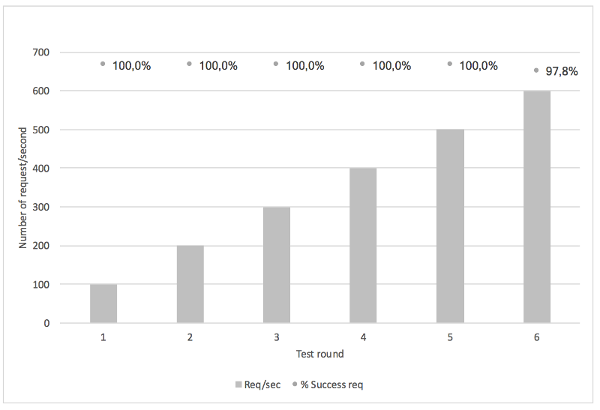
\includegraphics[scale=1]{fig/performance_1.png}
\DeclareGraphicsExtensions.
\caption{Predictor load test (reqs/second).}
\label{fig_load}
\end{figure}

\begin{figure}[h]
\centering
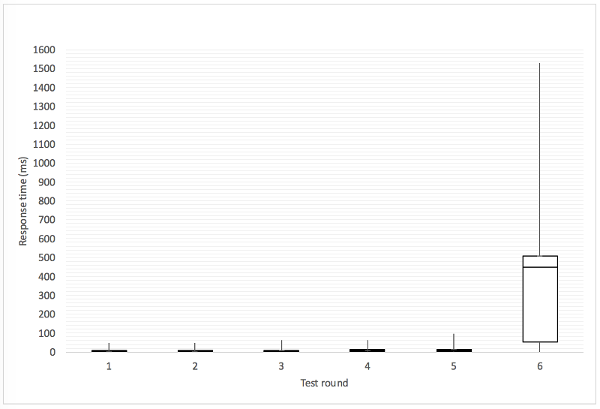
\includegraphics[scale=1]{fig/performance_2.png}
\DeclareGraphicsExtensions.
\caption{Predictor load test (Response time box plot).}
\label{fig_load_2}
\end{figure}

The experiment strategy was to keep the amount of resources available and increase the throughput of concurrent requests being sent to the server until a significantly increase on the response time or failed requests was observed. The requests from client to server were made through the REST HTTP protocol and the machines were located in the same physical data center. As it is possible to see in Figures \ref{fig_load} and \ref{fig_load_2}, we achieved 500 predictions per second maintaining a stable response time and none failed requests, at round 6 the mean response time increased significantly and the error rate has raised. The behavior of test round 6 indicates that we crossed the edge of efficient parallelism of Marvin's engine-executor predictions. Although we consider this a good number, we encourage administrators to deploy several instances of engine-executors behind a load-balancer when more than 500 predictions per second must be served.

\newpage
\section{Sample Engine}

Marvin applications are also labeled as engines. An engine is composed by the application's source code, a file containing parameters for the application and the metadata file. We encourage users to implement decoupled engines that are easy to maintain and less bug prone. To induce that we propose the DASFE design pattern (Figure \ref{fig_dase}). This pattern is strongly based on the DASE pattern~\citep{chan2013predictionio}, however we added the feedback phase on it. This evolution intends to enable the engine to receive input from external applications or users, this kind of feature allows the model to be modified online or add hooks to start a new training pipeline.

\begin{figure}[h]
\centering
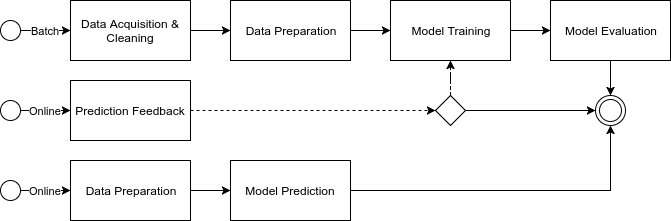
\includegraphics[scale=0.6]{fig/marvin-dase.png}
\DeclareGraphicsExtensions.
\caption{DASFE pattern pipeline.}
\label{fig_dase}
\end{figure}

We provide a project generator utility that generates the necessary base code for an engine, by doing that we reduced the complexity of the data scientist's job, requesting them to just populate these base files with the program logic. It is not necessary to care about passing the data to the next phase, or serializing the artifact in some persistence. 

The next paragraphs will present a simplified sample engine as reference. The sample is a Python engine able to classify products using a linear classifier with stochastic gradient descent (SGD). The engine uses a mix of Spark framework data structures and Pandas dataframe.

The code to obtain data from data sources and remove unnecessary rows, i.e. data cleaning, should be placed in the execute method of AcquisitorAndCleaner class:
\lstinputlisting[language=Python, frame=single]{code/acquisitor.py}

Then it is necessary to prepare the acquired data before training. The execute method on TrainingPreparator should contain preparation logic, e.g. inputation of missing values and data type transformation:
\newpage
\lstinputlisting[language=Python, frame=single]{code/training_preparator.py}

The model is finally trained at the Trainer class, when the execute method completes Marvin will serialize the model in the configured persistence:

\lstinputlisting[language=Python, frame=single]{code/trainer.py}

The MetricsEvaluator class is the appropriated class to place code related with model evaluation, in this example we're computing model error in a confusion matrix:

\lstinputlisting[language=Python, frame=single]{code/evaluator.py}

At PredictionPreparator the sample engine is just performing data transformation:
\lstinputlisting[language=Python, frame=single]{code/ppreparator.py}

Finally the Predictor class contains the logic that will be called for every valid http request made to the Predictor server:
\lstinputlisting[language=Python, frame=single]{code/predictor.py}

Deploying this code on Marvin's engine-executor will provide control over the training pipeline execution, dataframes and model serialization and versioning, metrics evaluation, model serving and feedback input interface.


\section{Conclusion}
Implement artificial intelligence applications with enterprise software characteristics is a hard task. Several contributions were made in libraries offering algorithms implementation and frameworks for distributed computing of data-intensive applications. Marvin add tools and integrate with libraries and data frameworks to support the exploration and model development of such kind of applications, it introduces a framework that speeds up the task of turning model prototypes into industry-grade software. Lastly Marvin's engine-executor is a model server that takes care of pipeline execution, artifacts serialization and offers a standard interface to allow other applications to access the model, it takes into account non-functional requirements to allow safe concurrency and effective parallelism on shared and distributed memory. The experiments demonstrated that engine-executor is able to serve 500 predictions per second while maintaining stable response time and 0 failed requests.

Marvin engines are helping companies like B2W Digital to be data-driven organizations, serving algorithms that can automate decisions such as optimizing its products prices to increase revenue, detecting frauds at the earliest stage and customizing sorting of many offers of the same product to customer clusters. The platform meshes the necessary components to empower data scientists pursuing to deliver production level applications that can support high throughput and process large datasets.


\newpage
% Manual newpage inserted to improve layout of sample file - not
% needed in general before appendices/bibliography.


\bibliography{references}

\end{document}